\documentclass{standalone}
\usepackage{tikz,tikz-3dplot}
\usepackage{tikzscale}
\usepackage{csvsimple}
\usepackage{bm}
\usepackage{pgfplots}
\usepackage{xcolor}
\pgfplotsset{compat=newest}

% MATLAB colors (lines)
\definecolor{c1}{rgb}{0, 0.4470, 0.7410} % blue
\definecolor{c2}{rgb}{0.8500, 0.3250, 0.0980} % orange
\definecolor{c3}{rgb}{0.9290, 0.6940, 0.1250} % yellow
\definecolor{c4}{rgb}{0.4940, 0.1840, 0.5560} % purple
\definecolor{c5}{rgb}{0.4660, 0.6740, 0.1880} % green
\definecolor{c6}{rgb}{0.3010, 0.7450, 0.9330} % light blue
\definecolor{c7}{rgb}{0.6350, 0.0780, 0.1840} % red

\begin{document}

% 2d plot
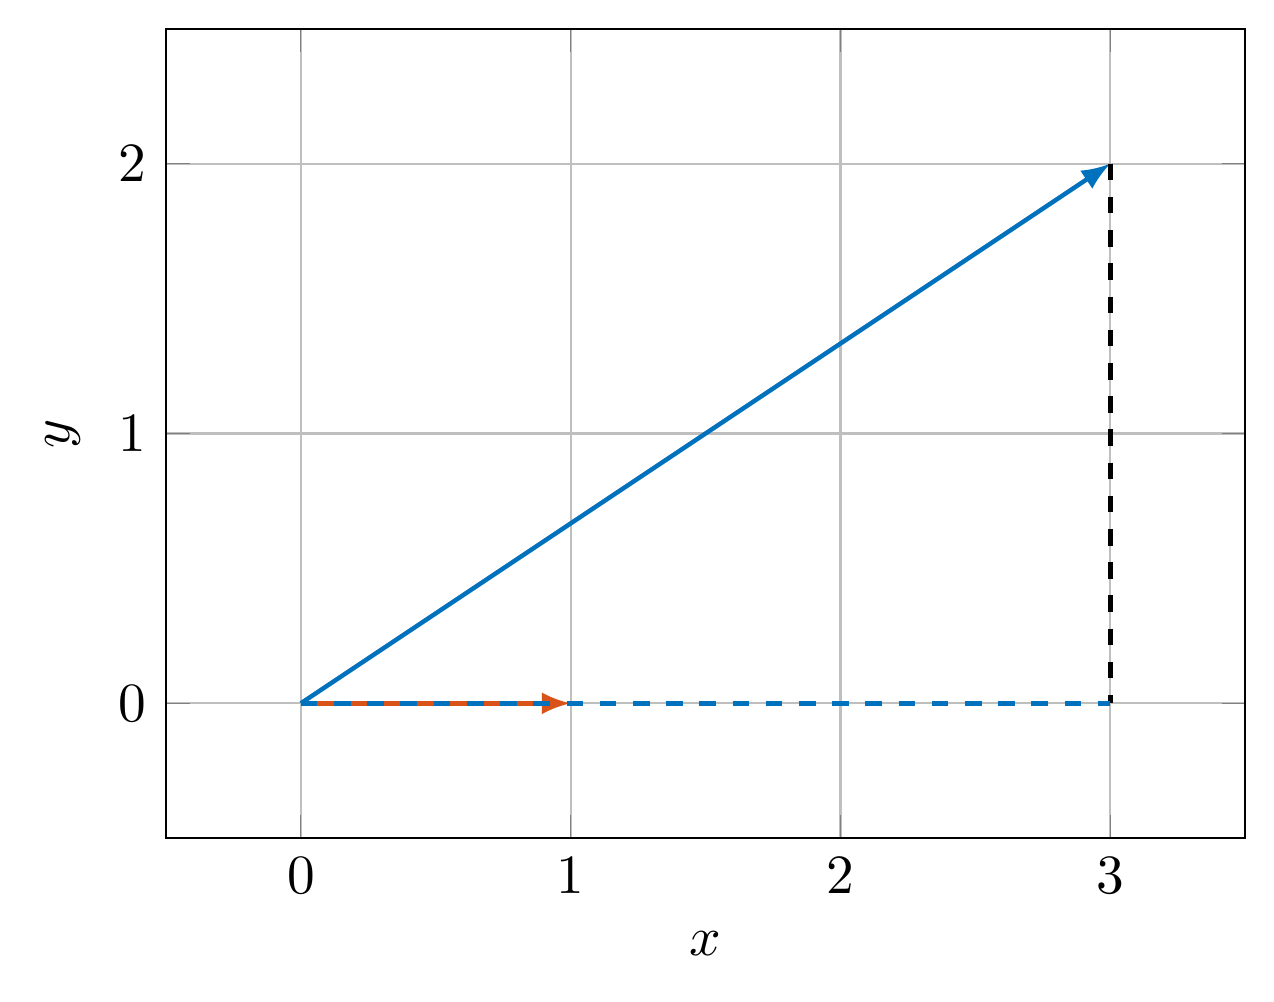
\begin{tikzpicture}[scale=2]
    \begin{axis}[
            xlabel=$ x $, ylabel=$ y $,
            xmin=-0.5, xmax=3.5,
            ymin=-0.5, ymax=2.5,
            grid, axis equal image,
            legend cell align=left,
            legend style={
                    at={(axis cs:3.5,2.5)},
                    anchor=north east,
                    font=\tiny,
                    draw=none,
                    fill=none
                }
        ]
        \addplot[-latex, c1, thick] coordinates {(0,0) (3, 2)};
        \addplot[-latex, c2, thick] coordinates {(0,0) (1, 0)};
        \addplot[dashed, black, thick] coordinates {(3,2) (3, 0)};
        \addplot[dashed, c1, thick] coordinates {(0,0) (3, 0)};
    \end{axis}
\end{tikzpicture}

\end{document}